\section{Object Detection and Instance Segmentation}

\subsection{任务简介}

\begin{figure}[htbp]
    \centering
    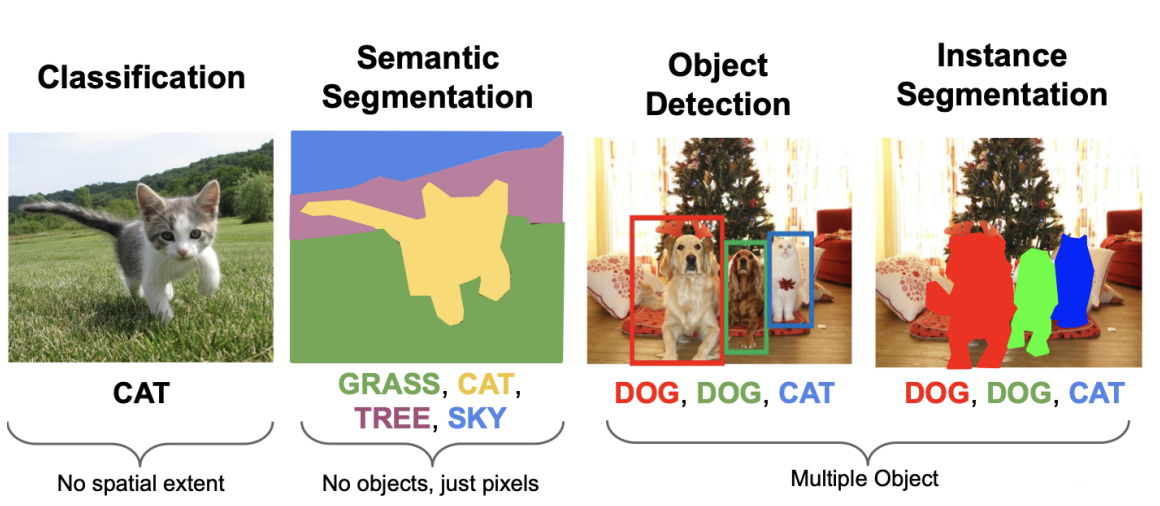
\includegraphics[scale=0.55]{figures/cv_tasks.png}
    \caption{分类任务}
\end{figure}

如上的任务当中,最左侧的是分类,即一张图片里只有一个待分类的事物.

随后是语义分割,即将代表不同语义的像素区分开来,每个像素都要有一个输出,
它不区分不同的个体.随后是目标检测,它区分不同个体,
但并不一定每个像素都被一个bounding box包围.

最后在此之上可以继续进行语义的分割.

\subsection{Object Detection: Single Object}

它的目标是定位和分类,
网络输出是2D的bounding box,且是axis aligned的.\footnote{到了三维的时候,
由于阶数的提升,axis-aligned bounding box中有非常多的部分并不属于这个物体,
因此可能需要旋转.但是对2D来说,这并不成为问题.}

确定bounding box需要四个参数
$x, y, w, h$,即bbox左上角的坐标和大小.\footnote{如果我们用八个点的坐标作为表示,
那么显然有很多冗余.尤其在高维的情形,如何找到冗余尽可能少而能够便利地表达
某一对象的方法是非常重要的.在后面的旋转部分,我们还会看到这一点.}

总的来说,单目标检测可以被划分成两个任务:(对图片的)\textbf{分类}和
(对bbox)的\textbf{回归}.如下图:

\begin{figure}[htbp]
    \centering
    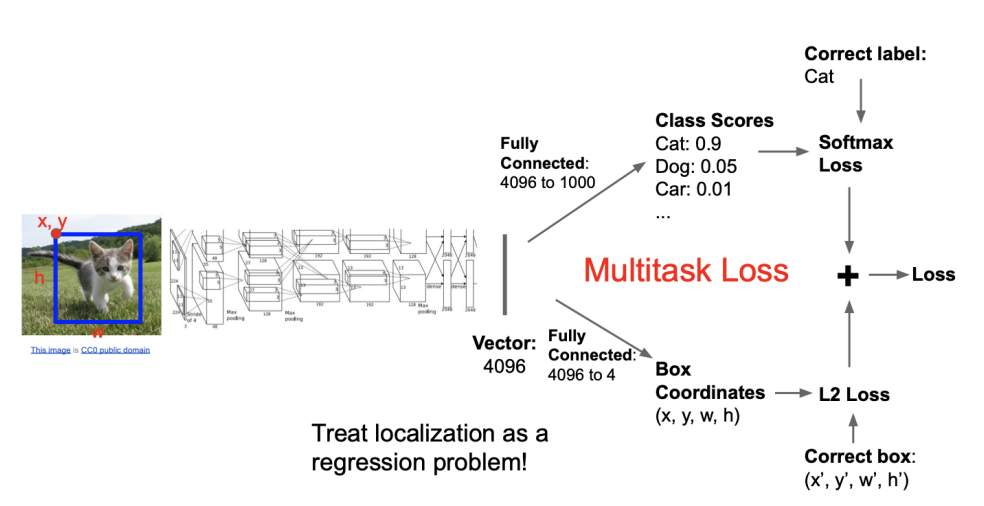
\includegraphics[scale=0.55]{figures/single_obj_det.png}
    \caption{单目标检测的网络概念图}
\end{figure}

假设我们得到了图片的特征向量,那么可以通过MLP变成分类概率的向量,
然后使用交叉熵进行度量;然后我们对图片MLP到四个数值,然后用$L^2$ 
loss进行回归

注意$L^2$ norm和 $L^2$ loss的区别:

$L^2$ norm是模长,$L^2$ loss是平方和.当$L^2$ norm作为损失函数时,
被称为rooted mean squared error(RMSE),而另一个则是mean squared error.

RMSE因为开根号的问题,在接近0时可能出现问题, 很少用.

MSE在接近收敛的时候,梯度也小,不容易越过, 同时MSE在较大的时候,梯度很大,
容易导致神经网络训练效果不好,而且还容易出现NaN.

\[\mathrm{smooth}_{L_1}(x)=\left\{\begin{array}{ll}0.5x^2&\mathrm{if}|x|<1\\|x|-0.5&\mathrm{otherwise}\end{array}\right.\]

Smooth L1 Loss:结合两者, 在较小的时候二次, 
在较大的时候一次, 同时加入常系数以保证一阶和二阶连续.

这是一个Multitask Loss,即分类loss和bounding box的loss之和,
可能产生竞争.它们应该以何种比例叠加?比如分类的loss最大大概在$\log N$的量级,
但是对bounding box来说,如果采用$L^2$,差5个pixel那就是25.而$e^{25}$
是一个非常大的数字.即使loss的量级差不多,gradient的量级也不一定是相同的.

除此之外,这个网络还有一个特殊性质:对于不同图片,可能需要不同数量的输出.
这在以前的Neural Network是无法做到的.

一个方法是用sliding window进行遍历检测,
但这也自然而然带来一个问题:不知道window多大, 并且计算量极大

后来的传统方法采用了Region Proposal的方法,即先提出一些可能是物体的bbox,
在其中进行检测.后来将这些proposal称为Region of Interest (RoI).

\subsection{Region-based CNN}

第一个深度学习的相关工作\cite{RCNN}:R-CNN (Region-based CNN).

它的大致流程是:先提出一些proposal,统一变换到224*224的大小,
然后通过SVM进行分类,以及对bbox的回归,
回归的输出是$(dx, dy, dh, dw)$,即bbox应该进行的调整.

\begin{figure}[htbp]
    \centering
    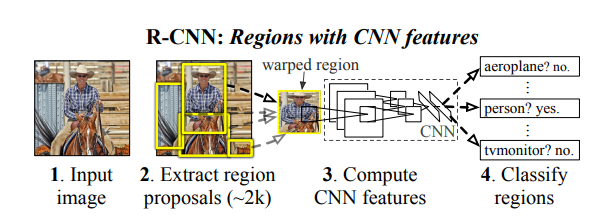
\includegraphics[scale=0.9]{figures/RCNN_classification.png}
    \caption{RCNN分类部分}
\end{figure}

训练时我们会有很多的RoI,但ground truth (后文简写成gt)的数量显然要少得多.
那么如何确定一个RoI被分成哪一类,以及向哪个gt进行回归呢?
首先,如果一个bbox与任何一个gt的交都小于某一阈值,那么就将它单独分类成background,
此时我们不再关心其regression的情况;如果一个bbox同时包含了多个gt,
那么可以计算它与这些gt的IoU,将IoU最大的那个gt作为其分类和回归的对象.
这里要注意的是,我们不关注background的回归是必须采取的行为,
因为如果要监督一个background的回归,那么它的loss是非常大的,会直接破坏其他RoI的训练.

做 research 一定要着眼于已有工作的不足,尤其是可以一眼看出来的问题.

这个工作的两个问题:

1. 首先proposal可能太多了,在测试时速度太慢.

2. 其次若给出的RoI比物体小,将其Crop之后的部分无法获知周围的信息,
几乎不可能准确对bbox进行回归.

\subsection{Fast R-CNN}

\begin{figure}[htbp]
    \centering
    \subfigure[取对应的bbox]{
        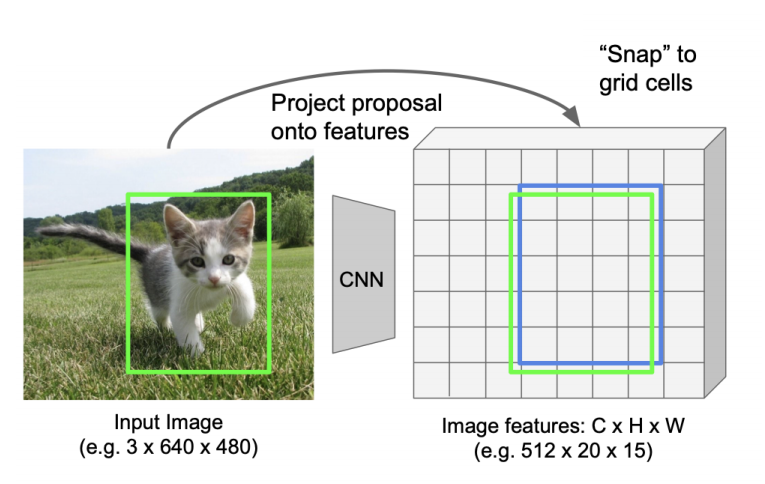
\includegraphics[scale=0.45]{figures/RoI_pool.png}
        \label{fig:get bbox in feature map}
    }
    \subfigure[RoI pool]{
        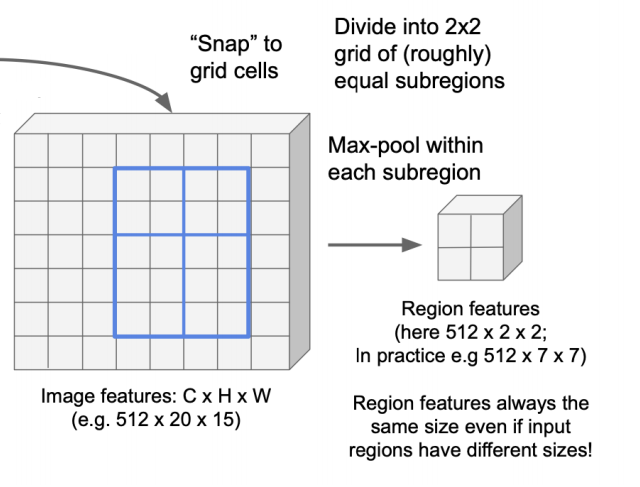
\includegraphics[scale=0.45]{figures/RoI_pool2.png}
        \label{fig:RoI_pooling}
    }
    \caption{Fast RCNN}
\end{figure}

随后提出的Fast R-CNN解决了上面的两个问题.

Fast RCNN仍然采用传统方法获得RoI,但是把Corp的时机放到了CNN之后.

将整个图片过CNN,再在feature map上取出对应的bbox.图像在卷积的过程中分辨率会减小,
因此在feature map上取的时候也要对应地缩小RoI,如图
\ref{fig:get bbox in feature map}所示,缩小过程中不在格点上的顶点被吸附到最近邻的
格点上.

这样取得的RoI大小仍然不统一,原论文采用了一种max pooling的方法,
将形式各异的RoI分割成合乎要求的子块,对每个子块求最大值,
如图 \ref{fig:RoI_pooling}所示.图中为方便将最终的大小画成了2*2,实际上为7*7.

这样做的好处是

1. 经过conv后,感受野也增大了,也就不会产生上文提到的被裁剪而缺少上下文的问题了

2. 因为最后特征图上的的RoI分辨率比较小,可以将多出来的RoI数量这一维度作为Batch的一部分,
从而可以完全并行化.使用32bits浮点数计算,
以每一个RoI对应的7*7*512的特征图为例,224的大小000个RoI,只需要不到200MB显存,
但是RCNN中2000个RoI,224*224*3的原始图片,需要1GB多的显存.

Fast RCNN相比RCNN取得了可观的速度提升.
如图,Fast RCNN的训练时间只有RCNN的约十分之一,且测试速度显著提高.
右图红色为不包含传统方法获得RoI,仅对RoI进行处理的时间,可以看出Fast RCNN
时间的限制在RoI的提出上了.

\begin{figure}[htbp]
    \centering
    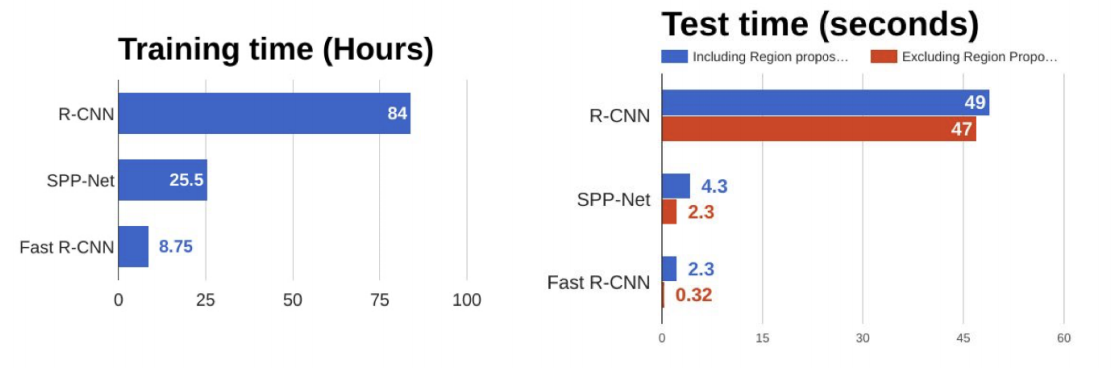
\includegraphics[scale=0.65]{figures/rcnn_vs_frcnn.png}
    \caption{RCNN v.s. Fast RCNN}
\end{figure}

\subsection{Faster R-CNN}

经过R-CNN和Fast R-CNN的积淀,Ross B. Girshick在2016年提出了新的Faster RCNN.

在结构上,Faster RCNN已经将特征抽取(feature extraction),proposal提取
都整合在了一个网络中,使得综合性能有较大提高,在检测速度方面尤为明显.

但是依然不是端到端的网络,还是一个两阶段的网络, 因为其中的proposal提取仍然需要首先训练.

\begin{figure}[htbp]
    \centering
    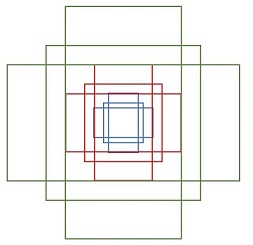
\includegraphics[scale=0.7]{figures/anchor.jpg}
    \caption{不同形状的anchor}
    \label{fig:anchor}
\end{figure}

首先引入Anchor box的概念, anchor box是一些预先定义好大小的bounding box,数量为K个.

如何提取proposal?在Fast R-CNN中,我们是通过Region Proposal Network(RPN)来提取的.

在Fast R-CNN中,我们已经得到了feature map,
而其中的每个pixel都可能作为不同形状的一个或多个物体的中心,因此我们可以
让每个pixel都给出自己是否是一些不同形状的anchor的中心(如图 \ref{fig:anchor}所示)
对于20*15*512的一张feature map得到20*15*K个概率值
这些300K个概率中最高概率的300个RoI将被作为最终输送给下一步骤的proposal.
所以第一步的batch size是图片数量, 第二步的batch size是图片数量*300.


当然,这样会获得数千个乃至更多的bbox,而一张图片里一般并没有这么多,在第二步完成之后还要进行优化.

1. 对于每个proposal,如果它在所有类上最高的概率小于某个阈值,则直接舍弃.

2. NMS.先将这些bbox进行分类预测,
按照它们的分类进行分组,随后对每个类型的分组内取分类概率最高的RoI,
将同组之内和它IoU大于某个threshold的RoI全部去除.
这样做的原理是将某一类别概率最高的作为标准,与其IoU较大的则认为是圈出了同一个物体,
全部去除;对于剩余的RoI重复这一操作.
\footnote{举例来说,假设猫分类的RoI中概率最大者圈住了一只猫的绝大多数,
因而以90\%的confidence认为是猫,则其他与它IoU大于
0.5的RoI很可能只圈住了这只猫的半边身子,
所以把它们都去掉.而IoU较小的可能是其他的猫.当然,这样做也存在一些问题,
比如有一个和它非常接近的RoI因为某种原因识别为狗,那么这样做就不能去除这样的RoI,
因为此处NMS只对同类的RoI进行操作.后来也有工作同时预测RoI与IoU(即"预测的预测"),
并证明这样做效果更优.}

\begin{wrapfigure}{r}{6cm}
    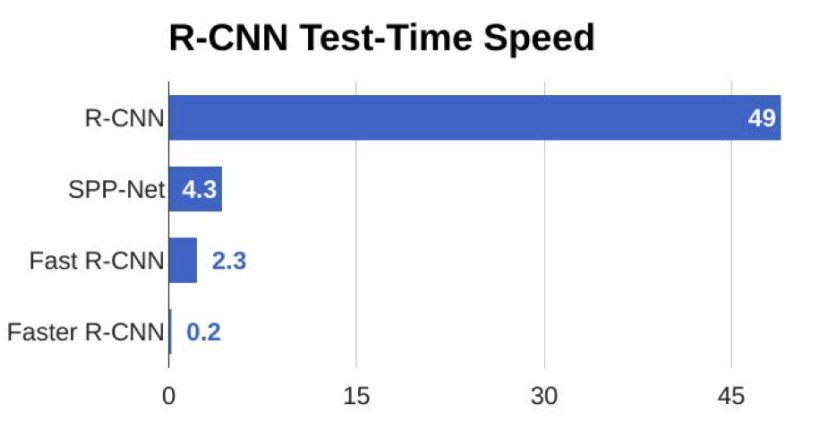
\includegraphics[scale=0.4]{figures/rcnn_speed_comparison.png}
    \caption{几种网络的速度比较}
    \label{fig:rcnn_speed}
\end{wrapfigure}

当然,Faster R-CNN之中还有非常多的细节,比如anchor如何取定,
如何确定训练RPN的positive/negative samples,如何参数化bbox回归的过程等,
限于篇幅限制无法一一展开,读者可参考\cite{FasterRCNN}.

Faster R-CNN中包含了四种loss:RPN对是否是物体的二分loss,
RPN regress box loss, final classification score, 
final box coordinates, 调参的过程自然是非常复杂的,
但是网络的效果也是显而易见的(如图 \ref{fig:rcnn_speed}).
Faster R-CNN的出现,使得目标检测不再是学术界的toy model, 
而是真正进入了实用领域,促进了安保等行业的发展.

\subsection{two-stage detector and one-stage detector}

\begin{figure}[htbp]
    \centering
    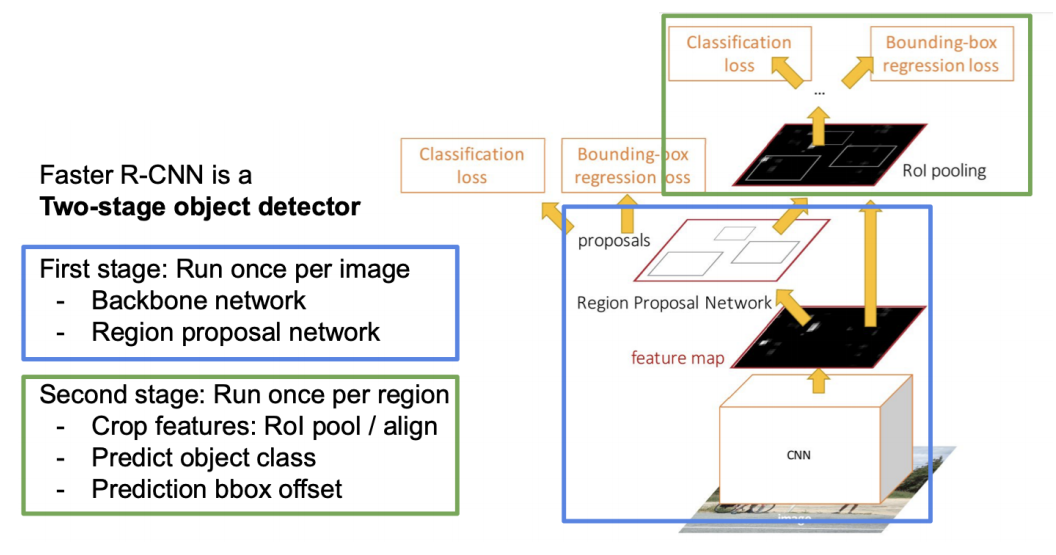
\includegraphics[scale=0.45]{figures/two_stage_detector.png}
    \caption{Two Stage示意}
\end{figure}

如上图,Faster R-CNN是一个分两步的目标检测网络.有人提出:
既然在第一步里也做了bbox 的refine,那么能否去掉第二步呢?这就诞生了single-stage 
detectors,代表有YOLO系列,它的特点就是非常快,目前能达到120 fps.
总体来说,two stage准确率占优,而one stage速度更快.

\subsection{Evaluation Metrics}

无论是一步还是两步,都需要面临的问题:我们如何评估预测结果?

% \marginpar{\kaishu 这是边注.这段话测试一下边注的分段和位置.    
% 庾信平生最萧瑟,暮年诗赋动江关.$$a = b$$}

AP (Average Precision): Precision-Recall curve 下的面积

假如我们有一张图,
有20个ground truth bounding box,我们显然不可能要求其完全相符.
我们可以定义一个IoU threshold.首先其输出的类别要对,其次IoU>threshold.
另外一方面,如果我乱猜了5000张,显然也是不行的.trade-off between
recall \& precision.因此提出度量:AP.即Average Precision.
即precision-recall图像下的面积.它先选出某个种类,然后按照prob排序,
逐个增加.这样precision下降,recall提升.mAP就是所有不同
category and/or IoU threshold.

AP at Different IoU Thres: 对于不同的IoU阈值,计算AP

mAP: 对于不同的 IoU Thres OR/AND 类别,计算AP,然后取平均

Object detection变量非常多.若要准确度,则Faster R-CNN.若要快速:
YOLO.但目前这一领域,工业界已经占据了统治地位.

\subsection{YOLO}

现在已经出到YOLO9了,但是这里只说最初的YOLOv1

\begin{figure}[htbp]
    \centering
    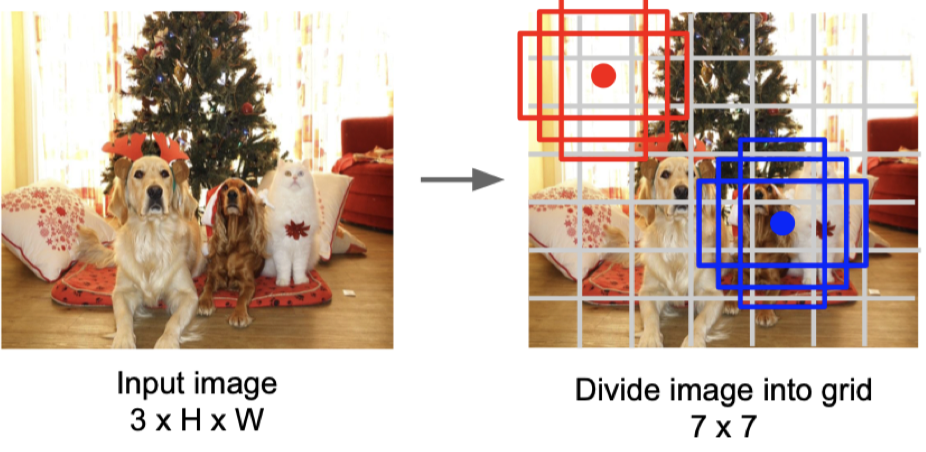
\includegraphics[scale=0.3]{figures/YOLO.png}
    \caption{YOLO}
    \label{fig:YOLO}
\end{figure}

将图片分为S*S个格子(一般S为7),每个格子负责预测她为中心的B个base boxes和C类.

所以输出为S*S*(B*5+C),其中5个值分别为:中心坐标,宽高,confidence.

\subsection{End-to-End Object Detection with Transformers (DETR)}

\begin{figure}[htbp]
    \centering
    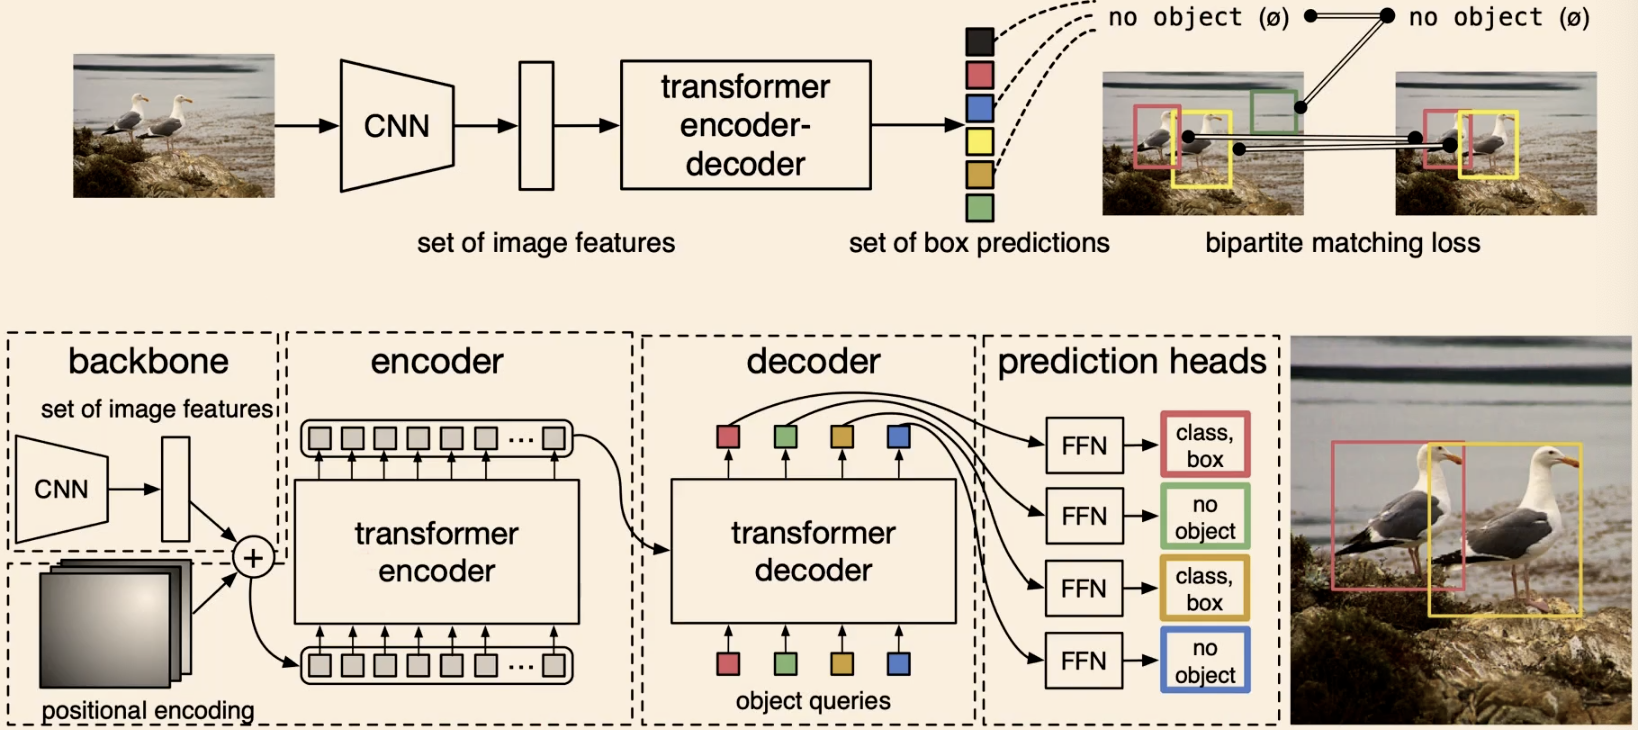
\includegraphics[scale=0.2]{figures/DETR.png}
    \caption{DETR}
    \label{fig:DETR}
\end{figure}



\subsection{考什么}

1. Transformer和Attention
2. NMS的过程, YOLO的metrics

\subsection{Mask R-CNN}

在目标bounding box检测上再进一步,输出哪个pixel属于哪个segmentation.
直接从box里出binary segmentation, 令人感觉trivial.

两种方法:bottom-up, top-down.目前在2D中前者较好,因为bbox已经做得很好.
后者在3D中有用.

Top-Down Approach:Mask R-CNN

何恺明是如何让这个看起来大家都看不起的工作拿到了ICCV 2017 best paper呢?
他在这篇文章中提出了RoI Align,Fast RCNN中从原始图片到feature map中的吸附
稍微丢失了信息, 所以边缘会很模糊.

首先,经过RoI pooling之后,分辨率可能下降.但这是大家都知道的.

\begin{figure}[htbp]
    \centering
    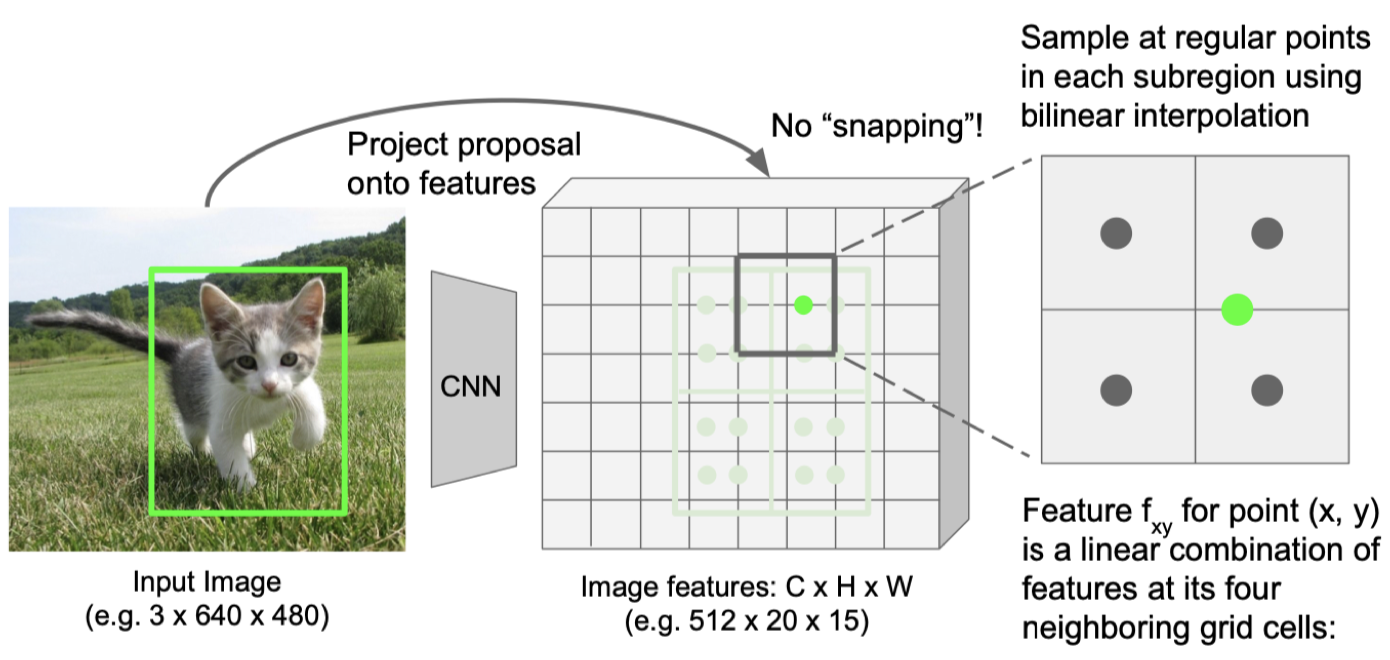
\includegraphics[scale=0.3]{figures/ROI_align.png}
    \caption{ROI align}
    \label{fig:ROI_align}
\end{figure}

最重要的在于,何恺明指出,我们不能进行最近邻的吸附,否则会不匹配,这是不可能被学习到的.
因此何恺明使用双线性插值进行处理,RoI align.

Ablation Study on RoI:
Align.AP at 75 提升比AP50还高,这是因为这样的方法对于高精度影响更大.
此外,加入align后,bounding box的表现也提升了, 这是因为RoI align后的特征更加精确.

\textbf{为什么Class-Agnostic Masks更好?}

猫的mask有猫的prior, 人的mask有人的prior, 因此通过预测所有类别的mask可以帮助前面的
网络学习bounding box和分类.

\subsection{3D Object Detection and Instance Segmentaiton}

期末考试不考

什么模态都有detection, 这里主要讲讲点云detection,对大模型之前的端到端自动驾驶很重要

三维axis align的bounding box自由度为6,orientated的为9.rotated bounding boxes
一般指只有y轴旋转的

三维一般需要考虑方向.

从2D到3D往往难度高很多.
